\documentclass[a4paper,11pt,fleqn]{scrartcl}%fleqn pour aligner les equations à gauche
\usepackage{../../Styles/Exercice}


\newcommand{\chnum}{Chapitre 15}
\newcommand{\chtitle}{Ondes Mécaniques}
\newcommand{\dtype}{Exercices}

\begin{document}
	\maketitle
\section{Calcul d'incertitude}
Une paroi rocheuse fait écho. Une randonneuse lance un appel et entend revenir son écho 6,0 s plus tard. À cette distance, l'incertitude est estimée à \SI{0,2}{s}. La célérité du son dans l'air est de \SI{330}{m.s^{-1}}.
\begin{enumerate}
    \item Faire un schéma de la situation.
    \item La distance $D$ qui dépare la randonnée de la paroi est comprise entre  une valeur $D_{min}$ et une valeur $D_{max}$ à cause de l'incertitude sur la durée. Calculer $D_{min}$ et $D_{max}$.
\end{enumerate}

% \begin{solution}
%     \item La distance $D$ qui sépare la randonneuse de la paroi est comprise entre  une valeur $D_{min}$ et une valeur $D_{max}$ à cause de l'incertitude sur la durée. Calculer $D_{min}$ et $D_{max}$.
%     \begin{align*}
%         D_{min} &= \frac{v \cdot (t - \Delta t)}{2} \\
%         D_{max} &= \frac{v \cdot (t + \Delta t)}{2}
%     \end{align*}
%     Avec :
%     \begin{itemize}
%         \item $v = 330 \, \text{m.s}^{-1}$
%         \item $t = 6,0 \, \text{s}$
%         \item $\Delta t = 0,2 \, \text{s}$
%     \end{itemize}
% \end{solution}

\section{Le cirque}
Un artiste de cirque veut faire claquer son fouet. Pour se faire, il génère, d'un mouvement de poignet, une "vague" qui se déplace à la célérité $v$ supposée constante le long du fouet.\\
On simule à l'aide d'un logiciel la perturbation le long de la lanière et on obtient la position de la vague à différentes dates séparées d'un intervalle de temps : $\Delta t = \SI{4,0}{ms}$ La lanière du fouet a une longueur de \SI{2,0}{m}.
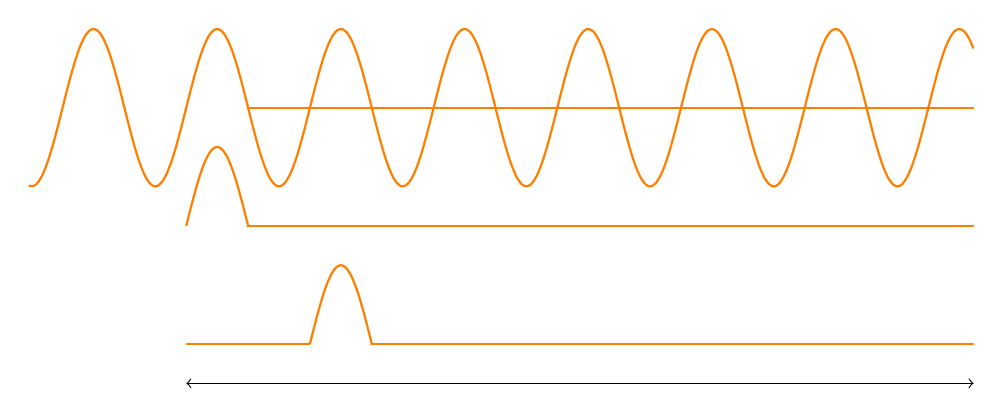
\begin{tikzpicture}
    \draw[<->] (0,0) -- (10,0);
    \draw[thick, orange] plot[domain=1.57:2.36,smooth] (\x,{.5+sin(4*\x r)});
    \draw[thick,orange] (0,.5)--(1.57,.5);
    \draw[thick,orange] (2.36,.5)--(10,.5);

    \draw[thick, orange] plot[domain=0:.79,smooth,samples=200] (\x,{2+sin(4*\x r)});
    \draw[thick,orange] (.79,2)--(10,2);

    \draw[thick, orange] plot[domain=-2:10,smooth,samples=200] (\x,{3.5+sin(4*\x r)});
    \draw[thick,orange] (.79,3.5)--(10,3.5);

\end{tikzpicture}
\begin{enumerate}
    \item Calculer la durée $\tau$ mise par l'onde pour parcourir la lanière du fouet.
    \item En déduire la célérité $v$ de l'onde.
\end{enumerate}
\end{document}